% !TEX root = Bachelorarbeit_Paul_Zilewitsch.tex
\section{Service Desk nach ITIL v3}

\subsection{Begriffsabgrenzung}

\noindent Für die Klärung des Begriffs \enquote{Service Desk} ist es sinnvoll, sich auf die Information Technology Infrastructure Libary - kurz ITIL - zu beziehen.
ITIL ist zwar keine Norm, die in der IT-Branche eingehalten werden muss, dennoch bezieht man sich im IT-Service Management ausschließlich auf ITIL.
Bereits 1989 wurde die Central Computer and Telecommunication Agency (CCTA) von der britischen Regierung beauftragt, Geschäftsprozesse und ihre Abhängigkeiten zu beschreiben und schriftlich festzuhalten.\footnote{Vgl. Olbrich, A. (2008): ITIL kompakt und verständlich, S.1.}
Ziel war es, Abläufe in der Unternehmenswelt darzustellen und dadurch die IT-Betriebskosten zu reduzieren. Im Laufe der Jahre wurden die ersten Ausarbeitungen überarbeitet und ergänzt. Die ITIL Edition 2011 ist die derzeitig neuste Fassung und stellt ein Update der 2007 veröffentlichten Version ITIL v3 dar.\footnote{Vgl. Vorlesung ITIL, S.25 5.Semester.}
Auch bestimmte Normen leiten sich aus dem ITIL-Rahmenkonzept ab. Der internationale Standard ISO/IEC 20000 beispielsweise basiert auf die Version ITIL v2 und definiert die Minimalanforderungen des IT-Service-Managements für Organisationen. \footnote{Vgl. Buchsein, R./Victor, F./Günther, H./Machmeier, V. (2008): IT-Management mit ITIL® V3, S. 5ff.}
ITIL kann deshalb als "Quasi-Standard" gesehen werden. Es ist ein  Best-Practice Leitfaden, der beschreibt "Was zu tun ist, aber nicht wie". Das macht deutlich, dass ITIL durchaus Handlungs -und Interpretationsspielraum zulässt, aber dennoch in einem vorher definierten Rahmen greifbar sein muss. Beschrieben wird ITIL v3 in fünf Büchern, auf die später noch eingegangen wird:

\begin{itemize}
\item Service Strategy
\item Service Design
\item Service Transition
\item Service Operation
\item Continual Service Improvement
\end{itemize}

\noindent
ITIL kann als Framework gesehen werden, mit dem Abläufe im Bereich IT Service beschrieben werden können. Genauer gesagt, spricht man IT Services Management, kurz ITSM. Hier werden alle Methoden erläutert, die nötig sind, um die bestmögliche Unterstützung von Geschäftsprozessen durch die IT-Organisation zu erreichen.\footnote{Vgl. Ebel ,N. (2008):  ITIL® V3 Basis-Zertifizierung, S.27 ff.} In ITIL ist ein Prozess ist definiert als \enquote{Satz von in Wechselbeziehung oder Wechselwirkung stehenden Tätigkeiten (und Mitteln), die Eingaben in Ergebnisse umwandelt. Zu den Mitteln können Personal, Einrichtungen und Anlagen, Technologie und Methodologie gehören. Eingaben für einen Prozess sind üblicherweise  Ergebnisse anderer Prozesse.}\footnote{Müller, A. (2015): Vorlesung ITIL, Skript S.18, 5.Semester.}\footnote{DIN EN ISO 9000:2005, Qualitätsmanagementsysteme , S. 23.}

\noindent
Jeder IT Service Management-Prozess hat eine charakteristische Zielrichtung und wird durch Funktionen unterstützt. Eine Funktion besteht aus einer Gruppe von Personen und deren Werkzeuge, die dafür verwendet werden, ein oder mehrere Prozesse oder Aktivitäten zu stützen.\footnote{ Vgl. Cannon, D./Wheeldon, D. (2007): Service Operation, S. 233.} Außerdem bewirkt das Zusammenspiel verschiedener IT Service Management-Prozesse, dass dem Kunden die notwendigen IT Services zur wirkungsvollen Unterstützung seiner Geschäftsprozesse geliefert werden. Der Service Lifecycle in Abbildung \ref{fig:ITIL_Lebenyzyklus} veranschaulicht genau diese Kernprozesse und Kernfunktionen, die ein IT-Prozess während seiner gesamten Lebensdauer besitzt. Die einzelnen Teilbereiche decken sich mit den zuvor aufgeführten Büchern von ITIL v3.\footnote{Vgl. Ebel,N. (2008):  ITIL® V3 Basis-Zertifizierung, S.27 ff.}

\begin{figure}[h!]
\centering
	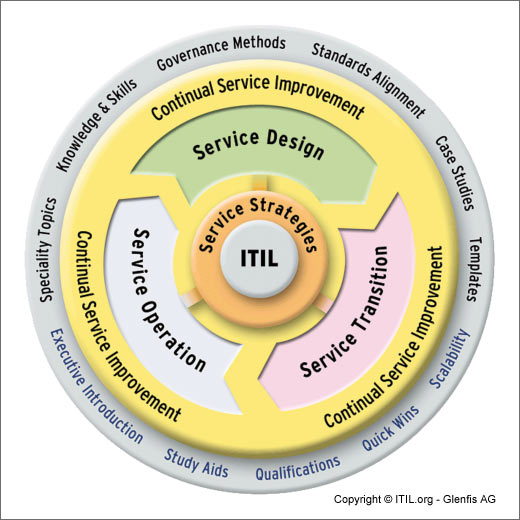
\includegraphics[width=0.50\textwidth]{Abbildungen/ITIL_Lebenszyklus}
	\caption[ITIL Service Lifecycle]{ITIL Service Lifecycle, Quelle: http://os.itil.org/osMedia/site/t1 
	media/JPEG/01\_itil\_imap.jpg}
	\label{fig:ITIL_Lebenyzyklus}
\end{figure}

\noindent
Auf alle Teilbeibereiche einzugehen, wäre zu zeitaufwendig, ist aber auch gar nicht nötig. Der Service Desk ist nämlich Bestandteil der Service Operation und somit die richtige Anlaufstelle für die Begriffsklärung. \newline \enquote{Service Operation beschreibt den Abschnitt des Lebenszyklus, der von den Kunden primär wahrgenommen wird.}\footnote{Vgl. Ebel, N. (2008): ITIL® V3 Basis-Zertifizierung, S.439.} In der Service Operations-Phase werden die Prozesse und Funktionen beschrieben, die einen stabilen  und bestmöglich IT Service garantieren sollen. Bei dieser Verbindung von IT Organisation und Kunde wird besonders auf den Kunden eingegangen. Der Service Desk ist hierbei \enquote{die zentrale Anlaufstelle, der Single Point of Contact (SPoC) zwischen Anwender und der IT-Organisation}\footnote{Vgl. Ebel, N. (2008): ITIL® V3 Basis-Zertifizierung, S.439.}. Wie der Name schon verrät, kommt der Anwender nur über diese Schnittstelle in Kontakt mit der IT. Hier werden Meldungen der Anwender üblicherweise erfasst, kategorisiert und eingetragen. Der Service Desk ist nicht nur eine Kommunikationsunterstürzung, sondern bietet gleichzeitig eine Auskunft für bereits bekannte Probleme. Dadurch kann bei häufig auftretenden Service-Unterbrechungen schneller gehandelt werden. Auch Supportanfragen, Beschwerden, Verbesserungsvorschläge oder Änderungswünsche können in den Service Desk eingetragen werden. Diese einzelnen Managementbereiche von ITIL v3 (Incident -, Problem -, Configuration -, Change -und Release Management) laufen im Service Desk zusammen, sodass der Benutzer nicht mehr entscheiden muss, in welchen Bereich sein Problem/Vorfall eingeordnet werden muss. Das ist dann Aufgabe des Supports. Die nachfolgende Abbildung verdeutlicht dieses Vorgehen.

\begin{figure}[h!]
\centering
	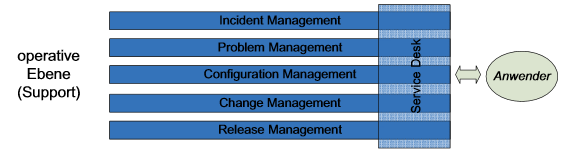
\includegraphics[width=0.75\textwidth]{Abbildungen/SPOC_2.png}
	\caption[Single Point of Contact]{Single Point of Contact, Quelle:http://edoc.hu-berlin.de/
	conferences/dfn2006/fischlin-roger-105/PDF/fischlin.pdf}
	\label{fig:ITIL_Lebenyzyklus}
\end{figure}

\subsection{Unterschied zu Help Desk}

\noindent
Bei der Begriffsabgrenzung zwischen Help Desk und Service Desk ist Vorsicht geboten. In mehreren Quellen ist zu finden, dass Help Desk (auch User-Help-Desk) lediglich ein veralteter Begriff für den Service Desk sei.\footnote{Vgl. Victor, F./Günther, H. (2005): Optimiertes
IT-Management mit ITIL, S.24.}\footnote{Meier, A./Myrach, T, (2004): IT-Servicemanagement, S.26.} Im Internet heißt es Beispielsweise auf Wikipedia: \enquote{Der Artikel Help desk und Service Desk überschneiden sich thematisch.}\footnote{https://de.wikipedia.org/wiki/Servicedesk, Stand 08.11.2013} In anderen Literaturquellen tritt der Begriff Help desk erst gar nicht auf oder wird dem Service Desk gleichgesetzt\footnote{Vgl. Olbrich, A. (2008): ITIL Kompakt und verständlich, S.19.}. Im Zweifelsfall sollte man sich direkt auf das Buch ITIL Service Operation beziehen. In dem heißt es übersetzt unter dem Stichwort Help Desk:
\enquote{Eine Anlaufstelle für Anwender, um Incidents zu erfassen. Ein Help Desk ist in der
Regel eher technisch orientiert als ein Service Desk und stellt keinen Single Point
of Contact für die gesamte Interaktion bereit. Der Begriff „Help Desk“ wird häufig
auch als Synonym für Service Desk verwendet.} \footnote{Vgl. Cannon, D./Wheeldon, D. (2007): Service Operation, S. 233. Übersetzung entnommen aus: Ebel, N. (2008): ITIL® V3 Basis-Zertifizierung, S. 699.} \newline
In den weiteren Ausführungen gilt deshalb der Help Desk als Synonym für den Service Desk.



\subsection{Anforderungen eines Service Desk}

\subsubsection{Aufgaben}
\noindent
Im folgenden sollen die wichtigsten Aufgaben eines Service Desk aus Sicht der ITIL v3 erläutert werden. Hierfür wird zunächst stichpunktartig die Kernaussage festgehalten, um sie anschließend zu erläutern. Dabei beziehen sich die Kernaussagen auf der Ausarbeitung Olbrichs aus \enquote{ITIL Kompakt und verständlich}
\footnote{Olrich, A. (2008): ITIL kompakt und verständlich, S.19 f.}
und sind eine leicht abgewandelte Form vom ITIL v3 Band Service Operation \footnote{Vgl. Cannon, D./Wheeldon, D. (2007): Service Operation, S. 110.}

\begin{itemize}
\item \enquote{Einheitlichen, zentralen Kommunikationsschnittstelle (SPoC) mit konkreten Ansprechpartner}
\end{itemize}
\noindent
Der Kunde hat mehrere Möglichkeiten den Support zu kontaktieren. Schreibt der Kunde eine E-Mail an den Support, könnte diese ausgewertet und den Service Desk eingetragen werden. Ebenso könnte er selbst einen Eintrag über ein Web-Frontend erstellen. Oder aber der Support erstellt einen solchen Eintrag im Service Desk, wenn der Kunde zum Telefon greift. Es ist aber Voraussetzung, dass eine einheitliche und zentrale Kommunikationsschnittstelle bereitgestellt wird.


\begin{itemize}
\item \enquote{Aufnahme, Dokumentation und Auswertung aller Vorfälle}
\end{itemize}
\noindent
Wenn alle Vorfälle ordnungsgemäß aufgenommen und dokumentiert wurden, kann schneller reagiert werden, wenn sich ein Problem wiederholt. Dass alle Vorfälle auch ausgewertet werden sollten, ist verständlich und kann eventuell dazu beitragen, Folgeprobleme frühzeitig zu erkennen.

\begin{itemize}
\item \enquote{Überwachung, Nachverfolgung und Eskalation von laufenden
Supportvorgängen. Frühzeitiges Erkennen von
Bedürfnissen und Problemsituationen}
\end{itemize}
\noindent
Wie im Punkt zuvor erwähnt können Probleme frühzeitig erkannt werden, indem Vorfälle genauestens ausgewertet werden. Das ist aber längst nicht die einzige Möglichkeit, Bedürfnisse der Kunden zu erkennen. Gute Mittel für vorausschauende Handlungen sind  bspw. Monitoring-Systeme oder log-Files. Sie liefern technische Informationen, die - nach einer Auswertung - Aufschluss über die aktuelle Lage des Kunden geben und in den Service Desk integriert werden könnten.


\begin{itemize}
\item \enquote{Überprüfung der Einhaltung des Dienstleistungsgegenstands
anhand von Service-Level-Agreements}
\end{itemize}
\noindent
Mithilfe des Service Desks kann kontrolliert werden, ob die vereinbarten Leistungen zwischen Auftraggeber und Beauftragter eingehalten wurden, wenn alle Vorfälle dokumentiert wurden.

\begin{itemize}
\item \enquote{Reporting – Beauskunftung gegenüber den Usern (Kunden)
und dem Management. Informationen über den aktuellen
Status von Vorgängen, geplanten Änderungen und
verschiedenen Nutzungsmöglichkeiten}
\end{itemize}
\noindent
Der Service Desk dient außerdem dazu, stets mit dem Kunden im Kontakt zu stehen. So können Information an den Kunden weitergeleitet oder auf der anderen Seite aktuelle Vorgänge, Status etc. des Kunden verfolgt und analysiert werden. 

\begin{itemize}
\item \enquote{Überprüfen der Kundenzufriedenheit, Stärkung der Kundenbeziehung.
Kontaktpflege. Aufspüren neuer Geschäftschancen}
\end{itemize}
\noindent
Nicht zuletzt kann der Service Desk auch als Instrument für einen ständigen Kontakt zum Kunden eingesetzt werden. Der Kunde hat dadurch den Eindruck, permanent mit der Support und somit der Firma verbunden zu sein. Das kann das Verhältnis zum Kunden stärken oder gar neue Geschäftsmöglichkeiten eröffnen.\\


\subsubsection{Kategorien}

\noindent
Grundsätzlich gibt es drei Kategorien bezüglich der Architektur eines Service Desks:

\begin{itemize}
\item Lokaler Service Desk
\item Zentraler Service Desk
\item Virtueller Service Desk
\end{itemize}

\noindent
Der lokale Service Desk zeichnet sich dadurch aus, dass er innerhalb eines Bereiches selbständig agiert. Mehrere Unternehmensstandorte oder verschiedene Bereiche eines Unternehmens haben jeweils einen eigenen Service Desk. Dieser kann präzise auf die Probleme und Prozesse vor Ort angepasst werden. Jedoch gestaltet sich eine Zusammenarbeit mehrere Bereiche gerade wegen dieser individuellen Service Desks schwierig. \\

\noindent
Beim zentralen Service Desk ist diese bereichsübergreifende Zusammenarbeit keine Hürde, da es einen Service Desk gibt, der für alle Bereiche eine gleichmäßige Zuständigkeit besitzt. Die Prozesse und Abläufe aller Benutzer sind hier identisch. Zwar sind die Kommunikationsmöglichkeiten hier sehr umfangreich, jedoch wächst die Informationsmenge rasant an. Eine kundennahe Betreuung wird durch den hohen Organisationsumfang deutlich erschwert. \\

\noindent
Bei der Kompromisslösung dieser beiden Architekturmodellen stößt man auf den virtuellen Service Desk. Die Informationseingabe der Benutzer kann durchaus an verschiedenen Standorten erfolgen ganz wie beim lokalen Service Desk. Doch alle Daten werden gesammelt und zentral verwaltet, was dem zentralen Service Desk entspricht. Entscheidend ist hierbei, dass es einheitliche Prozesse und Abläufe an den einzelnen Standorten geben muss. Individuelle Service Desks wären zu aufwendig in der Verwaltung. Auch so ist der Ressourcen -und Organisationsaufwand gegenüber den anderen Modellen enorm und bedarf guter Planung. \footnote{Vgl. Olbrich, A. (2008): ITIL kompakt und verständlich, S.21.} \footnote{Vgl. Cannon, D./Wheeldon, D. (2007): Service Operation, S. 111 f.} \\


\subsection{Analyse verschiedener Service Desk-Lösungen}

\subsubsection{Schwerpunkte der Analyse}

\noindent
Nach diesem sehr theoretischem Ansatz die Anforderungen eines Service Desks zu klären, wird nun auf Beispiele in der Praxis eingegangen. Wichtig sind dabei nicht Kriterien wie das äußere Erscheinungsbild oder die Kosten. Ziel soll es sein durch einen Vergleich gängiger Softwarelösungen, Verbesserungsmöglichkeiten der eigene Service Desk-Funktionalität in GEBman10 zu ermitteln. Dabei wird auf die drei folgenden Punkte Wert gelegt:

\begin{itemize}
\item Funktionalität:\\
		Die Funktionalität ist wohl das fundamentalste Kriterium. Hier ist entscheidend, welche 			
		Möglichkeiten dem Benutzer gegeben werden bspw. Meldungen/Tickets anzulegen, zu 
		zuweisen, zu suchen oder zu filtern. Wichtig ist aber auch, welche Informationen in welcher 
		Darstellungsform erhalten sind (Diagramme etc.) und welche Daten erfasst werden müssen 
		bzw. können.\\
		 
\item Bedienbarkeit:\\
		Aus diesem Blickwinkel wird untersucht, welche Bedienelemente zur Verfügung stehen. Eine	
		Bewertung nach intuitiver Bedienbarkeit ist schwierig vorzunehmen, da das immer eine
		subjektive Ansicht enthält.\\
		
\item Anpassbarkeit:\\
		Inwieweit kann man bspw. die grafische Oberfläche vom Benutzer geändert und auf die 
		eigenen Bedürfnisse angepasst werden.\\		
\end{itemize}


%hier sollte noch ein abschließender Satz hin



\subsubsection{Ausgewählte Service Desk-Lösungen}

\noindent
Nach den Recherchen auf mehreren Review und Ranking Websites zum Thema Service Desk / Help Desk, sind drei Softwarelösungen wiederholt erwähnt und gut bis sehr gut bewertet worden.\footnote{siehe Literaturverzeichnis}Diese drei webbasierten Anwendungen werden nun vorgestellt und anschließend ihre Stärken bzw. Besonderheiten dargelegt.

\begin{itemize}
\item Freshdesk:\\
		Girish Mathrubootham beschloss 2010 nach dem Lesen eines Nachrichtenartikels die Firma 
		Freshdesk ins Leben zu rufen. Das gleichnamige Produkt wird laut eigenen Angaben von rund 
		70.000 Kunden aller Unternehmensgrößen genutzt.\footnote{http://freshdesk.de/kunden/}
		\\
		 
\item Desk.com:\\
		Das Unternehmen Salesforce.com legt laut eigenen Angaben großen Wert auf mobile 
		Endgeräte und soziale Netzwerke. \footnote{http://www.salesforce.com/de/company/
		newspress/press-releases/2012/02/120201.jsp}Die Service Desk -Lösung des Unternehmens  
		nennt sich 	Desk.com und zu ihren Kunden zählen unter anderem die Firma FlixBus und die 
		Commerzbank.
		\\
		
\item Zendesk:\\
		Zendesk beschreibt sich selbst als \enquote{Kundenservice-Plattform}. Die gleichnamigen 
		Firma hat nach eigenen Angaben mehr als 75 000 Unternehmen, die diese Plattform nutzen. 
		Entstanden ist das Unternehmen 2007 aus einer Idee von drei Freunden aus Kopenhagen.
		\footnote{https://www.zendesk.de/about/}
		\\		
\end{itemize}

\noindent
Aktuell benutzt der Support von der KMS Computer GmbH die Software SysAid für den Service Desk. Durch eine Vielzahl von Einträgen und Erfahrungen der Mitarbeiter im Support, ist es sinnvoll auch diese Anwendung mit in den Vergleich einfließen zu lassen.

\begin{itemize}
\item SysAid:\\
		 Die Help Desk-Software SysAid wird nach eigenen Angaben in über 10 000 Unternehmen in 
		 140 Ländern eingesetzt. Die Firma SysAid Technologies wurde 2002 gegründet und zählt somit 
		 zu den erfahrenden Unternehmen dieser Branche.
		\\
\end{itemize}	

\noindent
Der Freshdesk besticht mit seinem sehr simplen Dashboard. Zur Erklärung: ein Dashboard ist üblicherweise eine kompakte meist grafisch aufbereitete Ansicht von Informationen.\footnote{https://help.salesforce.com/HTViewHelpDoc?id=bi_dashboard.htm&language=de} Der Benutzer erhält hier nur die wichtigsten bzw. neuesten Informationen. Auf den ersten Blick kann der Benutzer sehen, welche Tickets offen, nicht zugewiesen oder überfällig sind. Zusätzlich erhält der Benutzer die Möglichkeit, individuelle Aufgaben zu notieren und wie eine Checkliste abzuarbeiten. Ein sehr nützliches Feature für kleinere Notizen bzw. Probleme. Erst im zweiten Menüpunkt kann der Benutzer Tickets filtern. Hierfür gibt es gängige auswählbare Filter oder die Option einen Filter selbst zu konfigurieren und zu speichern.

\noindent
Vgl. IT Notfallmanagement unter Incident Management


\subsubsection{Zwischenfazit}